\documentclass[10pt]{article}
\usepackage[T1]{fontenc}
\usepackage[utf8]{inputenc}
\usepackage[margin=0.85in]{geometry}
\usepackage{amsmath}
\usepackage{booktabs}
\usepackage{array}
\usepackage{graphicx}
\usepackage{float}
\usepackage{placeins}
\usepackage{tabularx}
\usepackage{hyperref}
\graphicspath{{figures/}}

\title{Packet Tests of 2026-10-12:\\ How Trace Features and Images Respond to the Operating Parameters}
\author{ML-assisted optimization of CCD operating parameters --- working note}
\date{12 October 2026}
\newcommand{\code}[1]{\texttt{#1}}
\newcommand{\sep}{\mathcal{S}}

\begin{document}
\maketitle

\begin{abstract}
The run \code{2026-10-12-PA03\_PQ04\_Packet\_Tests} is the first with varied operating parameters. It has five settings:
the reference, VDD $-1.5$\,V, the vertical low rails and TG lowered, all horizontal low rails lowered, and only H3\_A\_L
lowered. Each setting has three trace sets (board 101, four channels), and the first four also have a 20$\times$20 binned image.
All 85 features of \code{src/trace\_features.py} were computed for every trace and compared between settings. The change was
measured in units of the scatter between the repeated trace sets.

Each parameter leaves its own fingerprint. The horizontal rails change the horizontal-transfer waveform (separation
$\approx$\,430). The vertical rails and TG change the vertical-transfer waveform ($\approx$\,340). VDD changes only the
amplifier response (settling time, pulse height and rise time). In the setting with the vertical rails and TG lowered, the
noise of amplifier A rises in both the trace and the image. A simple leave-one-out test assigns 46 of 47 trace sets to the
correct setting, so the features carry the operating parameters reliably.

The run is not enough to train a model of $\sigma_e$, $\lambda$ and the gain. It has 5 parameter sets with confounded
changes and no image labels. Section~\ref{sec:ml} lists what is needed.
\end{abstract}

\tableofcontents

%======================================================================
\section{The data}

The folder holds 378 files (3.9\,GB). For each setting there are 3 trace sets about 33\,s apart (2$\times$5 pixels, 500 skips,
20$\times$20 binning, 4 channels of board 101). They are followed about 3 minutes later by a synchronized image of boards 101 and
102 (50$\times$130 bins, 500 skips, 20$\times$20 binning, \code{EXPOSURE} 10\,s). Setting~5 has traces only, followed by an unfinished
pocket-pumping image. There are no packet manifests: the run was taken with the group's \code{take\_trace.py} /
\code{take\_image.py}, not with \code{take\_packet.py}. Only board 101 is analysed. In board 102's images, channels 0, 1 and 3
hold no charge.

\subsection{The settings}

The settings are read from the \code{.meta} files. Consecutive acquisitions with identical voltages and delays form one
setting (Table~\ref{tab:settings}, Figure~\ref{fig:settings}).

\begin{table}[H]
\centering
\begin{tabular}{llp{9.5cm}}
\toprule
Setting & Time (UTC) & Change from the reference \\
\midrule
1 reference & 18:56--19:03 & VDD $-19$\,V; V low rails 7.9/7.7\,V; H low rails 6.7/6.5\,V; TG 7.4\,V \\
2 VDD & 19:15--19:19 & VDD1, VDD2 $-19.01 \to -20.52$\,V (read back) \\
3 V low rails \& TG & 20:40--20:43 & V1\_A\_L, V3\_A\_L, V2\_C\_L $7.9\to7.4$; V1\_B\_L, V3\_B\_L $7.7\to7.2$; TG\_A\_H, TG\_A\_L, TG\_B\_H $7.4\to7.0$ \\
4 all H low rails & 20:59--21:02 & H1\_A\_L, H3\_A\_L, H2\_C\_L $6.7\to6.2$; H1\_B\_L, H3\_B\_L $6.5\to6.0$ \\
5 H3\_A\_L only & 21:09--21:15 & H3\_A\_L $6.7\to6.2$ \\
\bottomrule
\end{tabular}
\caption{The five settings (board 101). VDD returned to $-19$\,V after setting 2.}
\label{tab:settings}
\end{table}

\begin{figure}[H]
\centering
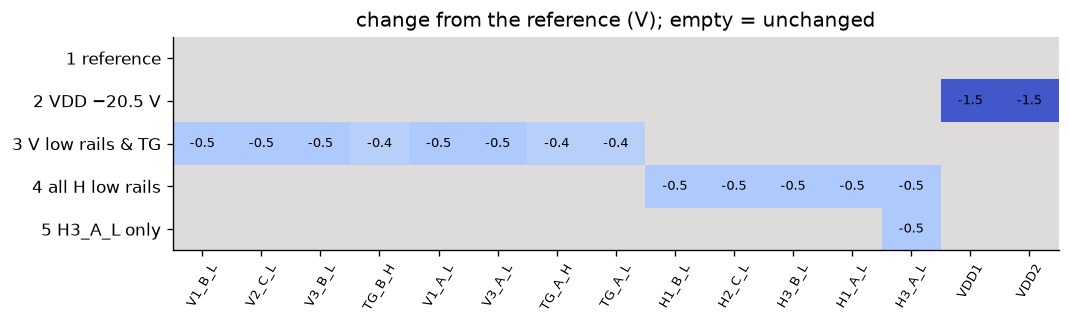
\includegraphics[width=0.85\textwidth]{oct12_settings.png}
\caption{Change of every varied parameter from the reference (V). Grey: unchanged.}
\label{fig:settings}
\end{figure}

\subsection{Things to know before comparing}

\begin{itemize}
\item \textbf{VDD returned to $-19$\,V after setting 2.} Settings 3, 4 and 5 differ from the reference in their rails only.
  The cleanest comparison is therefore \textbf{5\,$\to$\,4}: four horizontal low rails, nothing else. Next is
  \textbf{5\,$\to$\,3}: the vertical low rails and TG, plus H3\_A\_L going back up, which only affects the horizontal transfer.
\item \textbf{VDD has no clean comparison.} 1\,$\to$\,2 changes only VDD, but the traces of setting 1 were taken with a
  different trace setup (next item). 5\,$\to$\,2 has the same setup, but H3\_A\_L also changes. A feature is attributed to VDD
  only if it changes in the same direction in \emph{both}, and horizontal-transfer features are excluded.
\item \textbf{The traces inherited the image's prescan.} The traces of setting 1 have \code{NCOLPRE}\,=\,0 (0.8\,s, 12\,MB). All
  later traces have \code{NCOLPRE}\,=\,185 (1.7\,s, 68\,MB): \code{take\_trace.py} does not set the cuts, so it keeps those of
  the previous image. Each row then begins with about 3,720 horizontal transfers. Setting 1 is therefore a poor baseline.
\item \textbf{TG\_B on board 101 in setting 3 had its high level (7.0\,V) below its low level (7.4\,V).}
\item One trace (setting 5, channel 3, \code{\_211002\_91}) lost data and is refused by the quality check, leaving 59 traces.
\end{itemize}

%======================================================================
\section{Method}

For each trace, \code{trace\_features(trace, meta)} gives 85 numbers. These cover the horizontal and vertical transfer
waveforms, the skip cycle (reset pulse, summing-well dip, baseline droop), the amplifier response (fitted time constants,
pulse shape), the noise (CDS noise, spectra, Allan deviation, settling) and the levels. The analysis works for any trace
geometry, so the longer traces of settings 2--5 are handled correctly.

For a feature $f$ on one channel, with repeats $f_{a,i}$ in setting $a$ and $f_{b,j}$ in setting $b$, the
\emph{separation} is
\begin{equation}
\sep_{a\to b} = \frac{\bar f_b - \bar f_a}{s_\text{pooled}}, \qquad
s_\text{pooled}^2 = \frac{(n_a-1)s_a^2 + (n_b-1)s_b^2}{n_a+n_b-2},
\end{equation}
i.e.\ how many times larger the change is than the scatter between repeated trace sets. With 3 against 3 repeats,
$|\sep| \ge 6$ corresponds to $p \approx 0.002$ for one feature, so about 0.2 of the 85 features would pass by chance.
Figure~\ref{fig:example} shows what this looks like.

\begin{figure}[H]
\centering
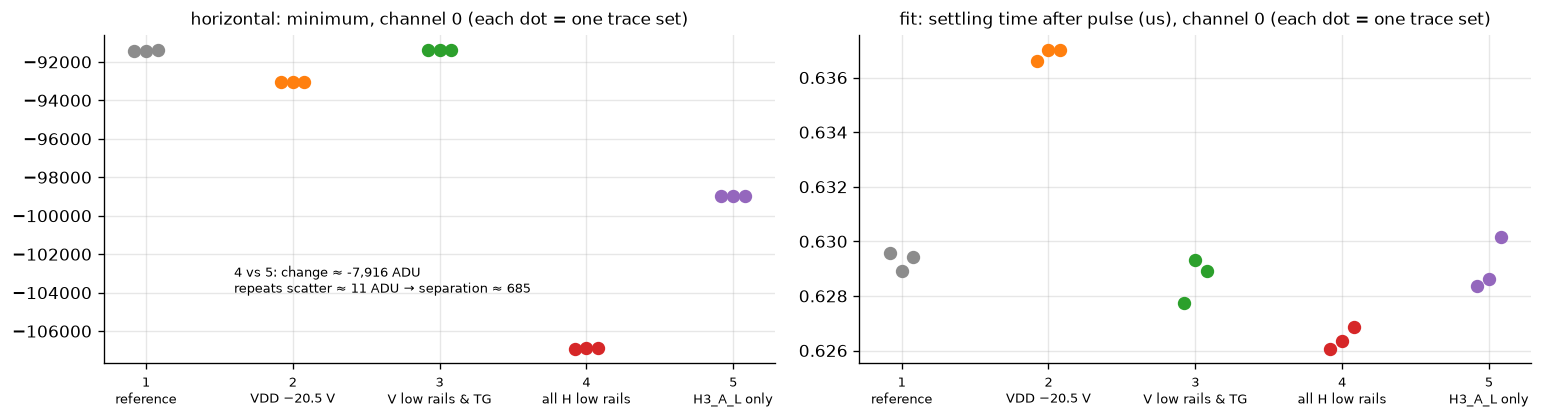
\includegraphics[width=\textwidth]{oct12_separation_example.png}
\caption{Two features on channel 0, each dot one trace set. Left: the lowest point of the horizontal-transfer waveform. The
repeats agree to about 11\,ADU and the settings differ by thousands (5\,$\to$\,4: $-7{,}900$\,ADU, separation $\approx$\,700
on this channel). Right: a subtle feature, the settling time after the reset pulse. The VDD change is only 0.008\,\textmu s,
but the repeats agree to about 0.001\,\textmu s.}
\label{fig:example}
\end{figure}

A feature counts as \emph{changed} by a parameter if it moves in the same direction on all four channels and the median
separation over the channels is at least 6. The features are grouped into five kinds: horizontal transfer, vertical transfer,
amplifier response, levels \& baseline, and noise \& fine structure.

%======================================================================
\section{Results: each parameter's fingerprint}

\begin{figure}[H]
\centering
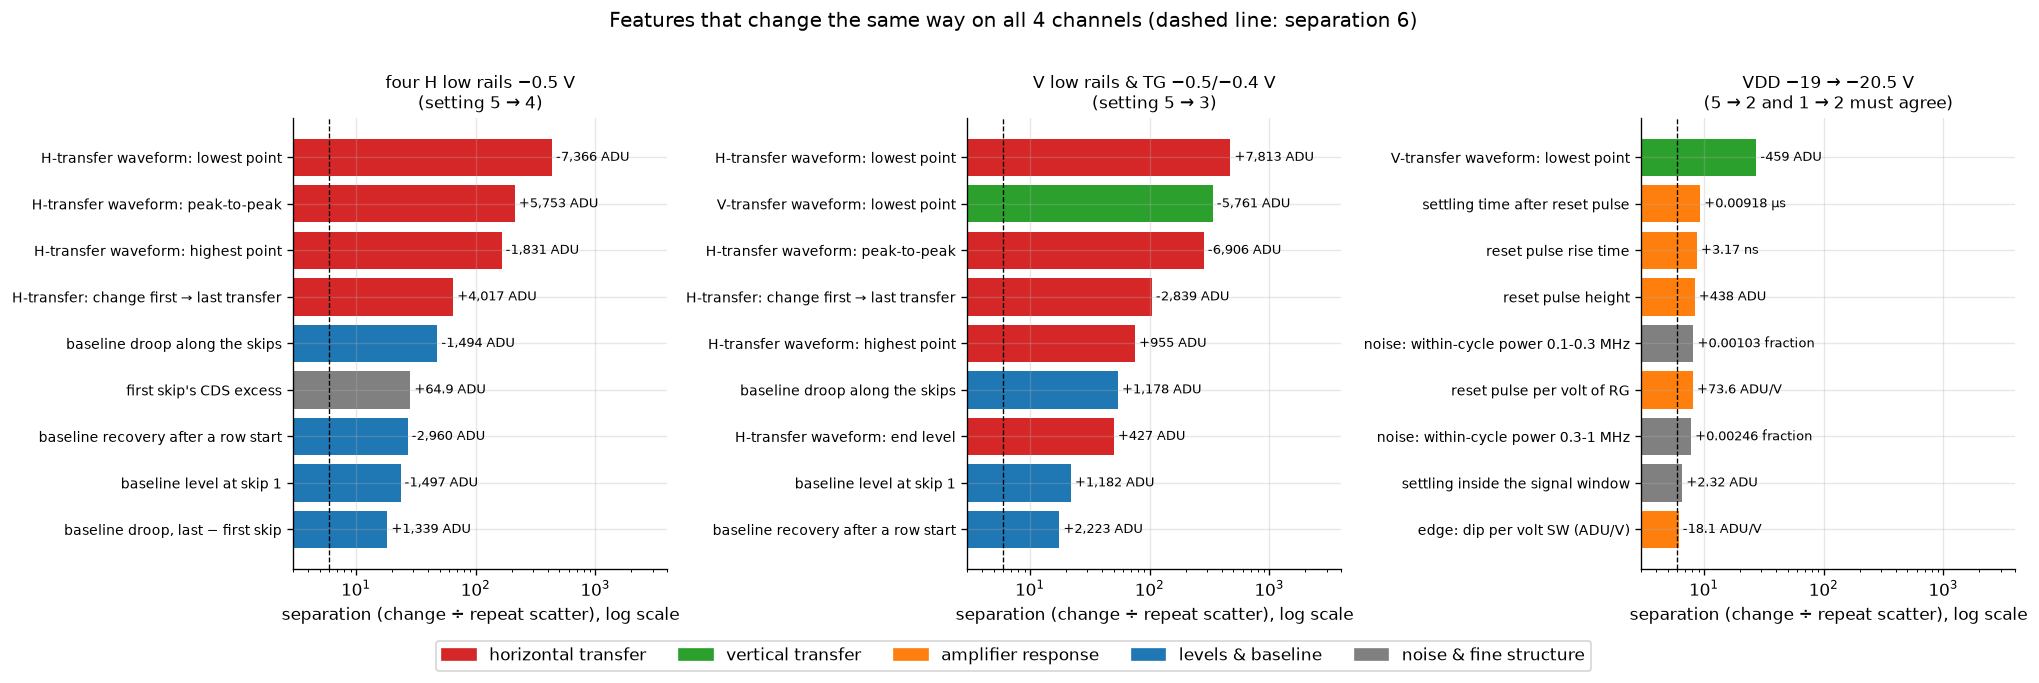
\includegraphics[width=\textwidth]{oct12_fingerprints.png}
\caption{The features changed by each parameter (same direction on all 4 channels, median separation $\ge 6$), ranked by
separation (log scale). The number at each bar is the median change over the channels. Colour: kind of feature.}
\label{fig:fingerprints}
\end{figure}

\begin{figure}[H]
\centering
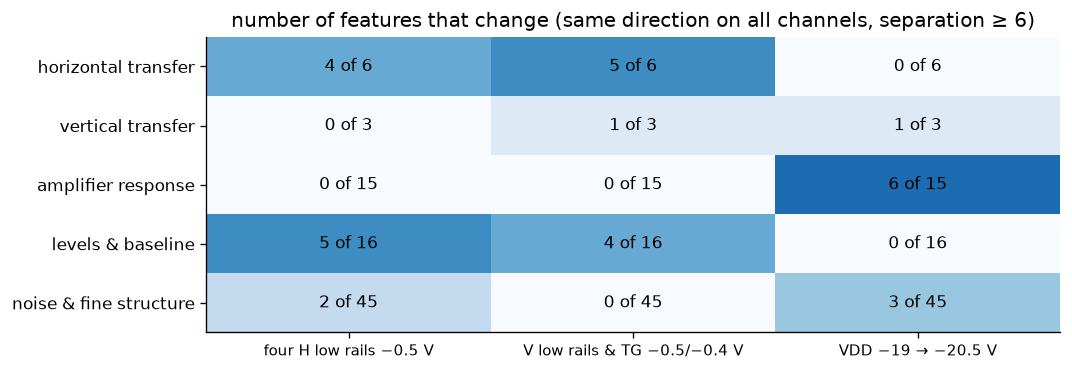
\includegraphics[width=0.75\textwidth]{oct12_feature_regions.png}
\caption{Number of changed features of each kind, per parameter change. Each parameter acts on a different part of the trace.}
\label{fig:regions}
\end{figure}

\begin{table}[H]
\centering
\begin{tabularx}{\textwidth}{lX}
\toprule
Parameter change & Main features changed (median over the channels; separation in brackets) \\
\midrule
Four H low rails $-0.5$\,V (5\,$\to$\,4) &
H-transfer lowest point $-7{,}370$\,ADU (430); H-transfer peak-to-peak $+5{,}750$\,ADU (210); H-transfer highest point
$-1{,}830$\,ADU (160); change first$\to$last transfer $+4{,}000$\,ADU (65); baseline droop $-1{,}490$\,ADU (48); baseline at
skip 1 $-1{,}500$\,ADU (24); row-start recovery $-2{,}960$\,ADU (27). \emph{No amplifier-response feature changes.} \\
\addlinespace
V low rails \& TG (5\,$\to$\,3) &
V-transfer lowest point $-5{,}760$\,ADU (340); baseline droop $+1{,}180$\,ADU (54); baseline at skip 1 $+1{,}180$\,ADU (22).
The H-transfer features also change (lowest point $+7{,}800$\,ADU), because H3\_A\_L goes back up in this comparison. \\
\addlinespace
VDD $-19\to-20.5$\,V (5\,$\to$\,2 and 1\,$\to$\,2 agree) &
Settling time after the reset pulse $+0.009$\,\textmu s (10); reset-pulse rise time $+3$\,ns (9); reset-pulse height
$+440$\,ADU (9); pulse per volt of RG $+74$\,ADU/V (8); V-transfer lowest point $-460$\,ADU (28); small changes of the
within-cycle noise spectrum. \emph{No horizontal-transfer feature changes.} \\
\bottomrule
\end{tabularx}
\caption{Fingerprints of the three parameter changes.}
\label{tab:fingerprints}
\end{table}

\paragraph{Interpretation.}
\begin{itemize}
\item \textbf{Horizontal low rails} deepen every negative swing of the horizontal-transfer waveform. Through the following
  baseline, they also shift the level and the droop of the skips. Lowering only H3\_A\_L (setting 5) gives about half of the
  effect of lowering all five rails, and only on the swings driven by that phase.
\item \textbf{Vertical low rails and TG} deepen the first part of the vertical-transfer waveform by about 5,000\,ADU.
\item \textbf{VDD} (an output-stage bias) changes only the amplifier: the reset pulse becomes higher and slower and settles
  more slowly. The transfer waveforms are almost unchanged. The changes are small in absolute terms, a few hundred ADU on a
  46,000\,ADU pulse, but 8--10 times the repeat scatter.
\end{itemize}

\begin{figure}[H]
\centering
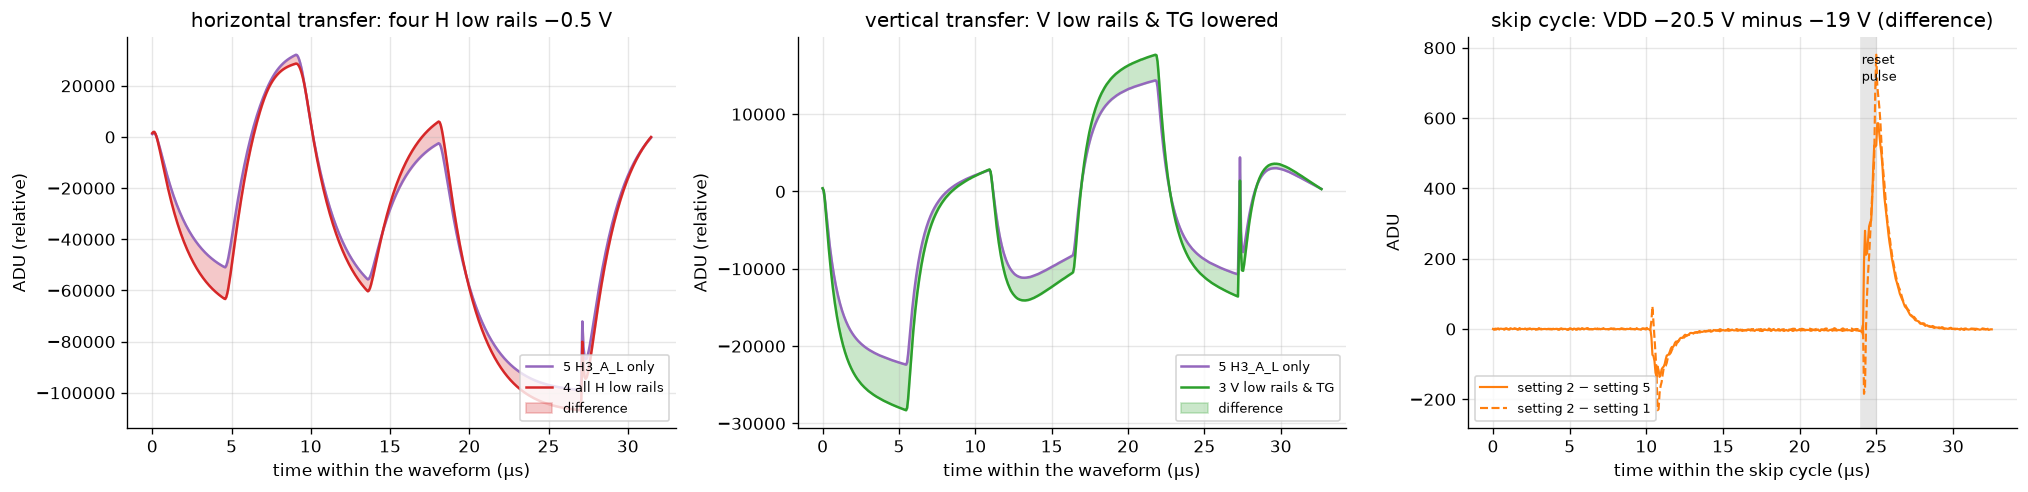
\includegraphics[width=\textwidth]{oct12_waveforms.png}
\caption{Mean waveforms, channel 0. Left: horizontal transfer, settings 5 and 4 (four H low rails). Middle: vertical transfer,
settings 5 and 3 (V low rails \& TG). Right: the VDD effect is too small to see on the raw curve, so the difference of the
mean skip cycles is shown, from both VDD comparisons. They agree: a higher pulse and a slower tail after the reset (grey
band).}
\label{fig:waveforms}
\end{figure}

%======================================================================
\section{Noise and the images}

\begin{figure}[H]
\centering
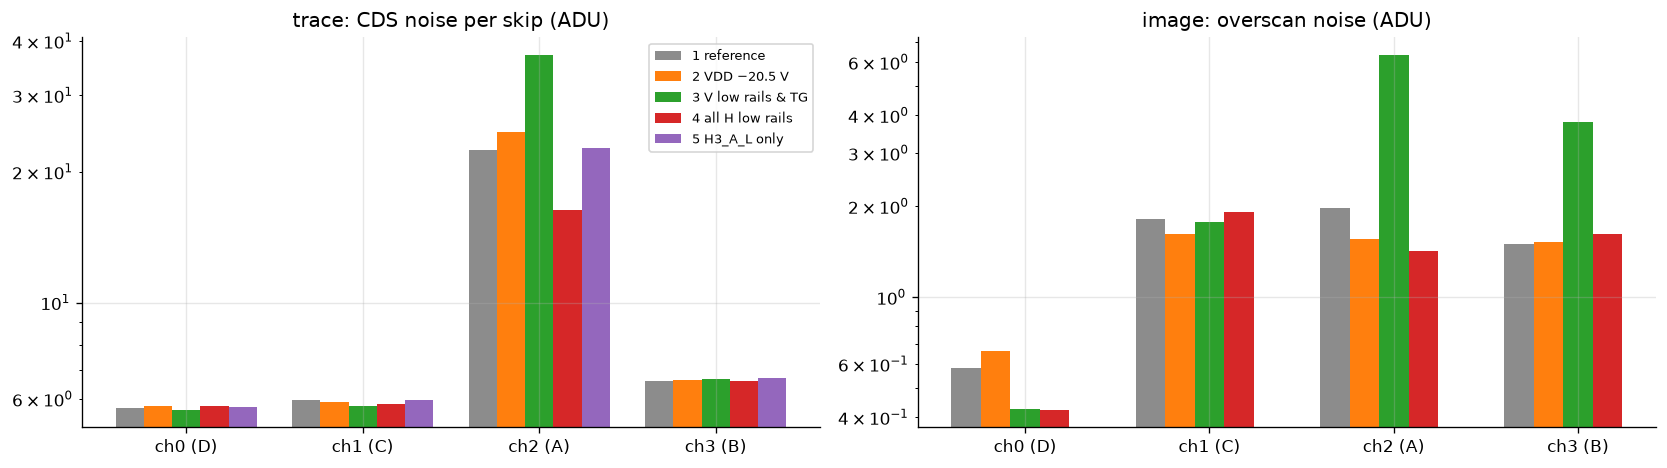
\includegraphics[width=\textwidth]{oct12_noise_trace_and_image.png}
\caption{Left: trace CDS noise per skip. Right: image overscan noise (robust scatter of the last 6 columns, 500-skip
average). Only settings 1--4 have images. Log scales.}
\label{fig:noise}
\end{figure}

\begin{table}[H]
\centering
\small
\begin{tabular}{lcccc}
\toprule
 & ch0 (D) & ch1 (C) & ch2 (A) & ch3 (B) \\
\midrule
Noise (ADU), settings 1/2/3/4 & 0.58/0.66/0.43/0.42 & 1.81/1.62/1.78/1.91 & 1.98/1.55/\textbf{6.35}/1.42 & 1.50/1.52/\textbf{3.80}/1.62 \\
Level change, setting 3 & $+0.3$ & $+0.3$ & $\mathbf{+10.9}$ & $\mathbf{+4.4}$ \\
Level change, setting 4 & $-1.3$ & $-1.9$ & $-1.3$ & $-1.2$ \\
Charge per bin (ADU), setting 1 & 27.2 & 29.5 & 42.9 & 37.4 \\
\bottomrule
\end{tabular}
\caption{Image overscan results, board 101 (level changes relative to setting 1, in ADU).}
\label{tab:images}
\end{table}

\begin{itemize}
\item \textbf{Channel 2 (amplifier A) is the noisiest} at every setting: 16--37\,ADU per skip in the trace, against about
  5.7\,ADU on channel 0.
\item \textbf{Setting 3 (V low rails \& TG, with TG\_B inverted)} raises the noise of channel 2 in \emph{both} the trace
  ($25\to37$\,ADU) and the image ($1.6\to6.3$\,ADU). The image of channel 3 is affected as well ($1.5\to3.8$\,ADU), and the
  overscan level of both rises. This is the first direct link between a trace feature and an image quantity.
\item \textbf{Setting 4 (H low rails)} lowers the overscan level of every channel by 1.2--1.9\,ADU, matching the baseline
  shift seen in the traces.
\item \textbf{The charge per bin barely changes.} With 20--35\,e$^-$ per 20$\times$20 bin (collected during the readout), WADERs
  cannot fit these images, so no $\sigma_e$, $\lambda$ or gain labels are available.
\end{itemize}

%======================================================================
\section{Could an ML model be trained on this?}
\label{sec:ml}

\subsection{Two different questions}

``Training a model'' can mean two different things here, and this run answers them differently.

\begin{enumerate}
\item \textbf{Are the trace features informative?} If a parameter is changed, do the features change in a reproducible
  way, so that a model could learn from them? This is a property of the \emph{inputs}, and it can be tested with this run
  (Sections~\ref{sec:ml-test}--\ref{sec:ml-pca}).
\item \textbf{Can we train the model we actually want?} That model takes the operating parameters $\theta$ (the $\sim$40
  voltages and delays) and the trace features, and predicts the image quality: the read noise $\sigma_e$, the dark current
  $\lambda$ and the gain, measured on the images with WADERs. An optimizer would then use it to propose better $\theta$.
  This needs many examples of ($\theta$, trace features, image labels), which this run does not have
  (Section~\ref{sec:ml-target}).
\end{enumerate}

\subsection{Test 1: can the features tell the settings apart?}
\label{sec:ml-test}

\paragraph{Idea.} If the features record the operating parameters, then a trace set whose setting is hidden can be assigned
to the right setting just by comparing its features with those of the other trace sets. This is the simplest possible
``model'' (a nearest-centroid classifier). If even this fails, a more complex model will not do better with so few examples.

\paragraph{Data.} Settings 2--5 only, because setting 1 used a different trace setup (\code{NCOLPRE}) and would be
recognised for that reason alone. Per channel there are 4 settings $\times$ 3 trace sets $= 12$ trace sets (11 on channel 3,
where one trace was damaged), 47 in total over the 4 channels. Each trace set is a list of 83 numbers: the 85 features, minus
2 that are undefined (NaN) for these traces. Each channel is tested separately.

\paragraph{Procedure (leave-one-out).} For each trace set in turn:
\begin{enumerate}
\item \textbf{Hide it.} The remaining 11 trace sets are the ``training data''.
\item \textbf{Average per setting.} For each setting, average the features of its remaining trace sets (3, or 2 for the
  setting of the hidden one). This gives one ``centre'' per setting: a list of 83 typical values.
\item \textbf{Put all features on the same scale.} The features have different units (ADU, \textmu s, ratios), so each is
  divided by its \emph{repeat scatter}: the standard deviation of the trace sets around their own setting's centre,
  pooled over the 4 settings. A difference of 1 in these units means ``as large as the difference between two repeats''.
\item \textbf{Measure the distance} from the hidden trace set to each centre. For feature $k$ and setting $g$:
  \begin{equation}
  z_{k,g} = \frac{x_k - c_{k,g}}{s_k}, \qquad d_g = \operatorname{median}_k\, z_{k,g}^2 ,
  \end{equation}
  with $x_k$ the hidden trace set's feature, $c_{k,g}$ the centre of setting $g$ and $s_k$ the repeat scatter.
\item \textbf{Assign} the hidden trace set to the setting with the smallest distance, and check whether that is its true
  setting.
\end{enumerate}

\paragraph{Example.} Hide one trace set of setting 4 (channel 0). For the lowest point of the horizontal-transfer waveform,
the repeat scatter is about 11\,ADU. The hidden value lies within a few ADU of the setting-4 centre ($z \approx 0$–1), but
about 7,900\,ADU from the setting-5 centre ($z \approx 700$). Most of the other features give the same verdict, so the
median distance is smallest for setting 4.

\paragraph{Result.} \textbf{46 of 47 trace sets are assigned to the right setting} (channel 0: 11/12; channels 1 and 2: 12/12;
channel 3: 11/11). Guessing would give about 1 in 4. The one mistake is a setting-5 trace set on channel 0, assigned to setting
3. Setting 5 is also the loosest cluster on channel 0 in Figure~\ref{fig:space}.

\paragraph{Why the median and not the sum.} With the \emph{sum} of $z^2$ over the features there are 3 mistakes (channels 1
and 3). The reason is the small number of repeats. After hiding one trace set, a setting may have only 2 repeats left. For
some feature, the repeats can then agree much better than usual \emph{by chance}, so its scatter $s_k$ is underestimated.
That feature's $z^2$ becomes huge for every trace set that is not exactly on its centre, and in a sum over 83 features this
one feature decides the result. The median ignores such outliers: it asks what the \emph{typical} feature says. In practice,
the model will need either robust weighting or a selection of reliable features, and more repeats per setting to estimate
the scatter well. The planned packets have 3 reference and 3 $\theta$ trace sets.

\paragraph{What this result does and does not show.} It shows that the features change reproducibly with the operating
parameters: the information is there. It does \emph{not} show that the features predict $\sigma_e$ or $\lambda$. Telling
apart 4 settings that differ by 0.5--1.5\,V is an easy task. It is a necessary condition for the real model, not a
sufficient one.

\subsection{Test 2: a picture of the feature space}
\label{sec:ml-pca}

Each trace set is a point in an 83-dimensional space (one axis per feature), which cannot be drawn. A
\emph{principal-component analysis} (PCA) finds the two directions along which the trace sets differ most, and
Figure~\ref{fig:space} shows the trace sets projected onto them:
\begin{itemize}
\item Each feature is first standardized (its mean over the 12 trace sets subtracted, divided by its standard deviation), so
  that no feature dominates because of its units.
\item PC1 is the combination of features with the largest spread between the trace sets; PC2 the next largest, independent
  of PC1. The percentages on the axes say how much of the total spread each direction holds (34\,\% and 20\,\% on channel 0).
\item The axes have no units. Only distances matter: \textbf{points close together have similar features}.
\end{itemize}

\paragraph{Reading the figure.} The 3 trace sets of each setting lie close together, and the settings are far apart: the
repeats are much more alike than the settings. PC1 roughly orders the settings by how much the horizontal low rails were
lowered: setting 4 (five rails) on the right, setting 5 (one rail) in between. PC2 separates setting 2 (VDD, top) from
setting 3 (V rails and TG, bottom). Setting 5 is the loosest cluster on channel 0, consistent with the one mistake of Test 1 being a
setting-5 trace set. Channel 2, the noisiest amplifier, looks the same. Its higher noise does not hide the setting differences.

\begin{figure}[H]
\centering
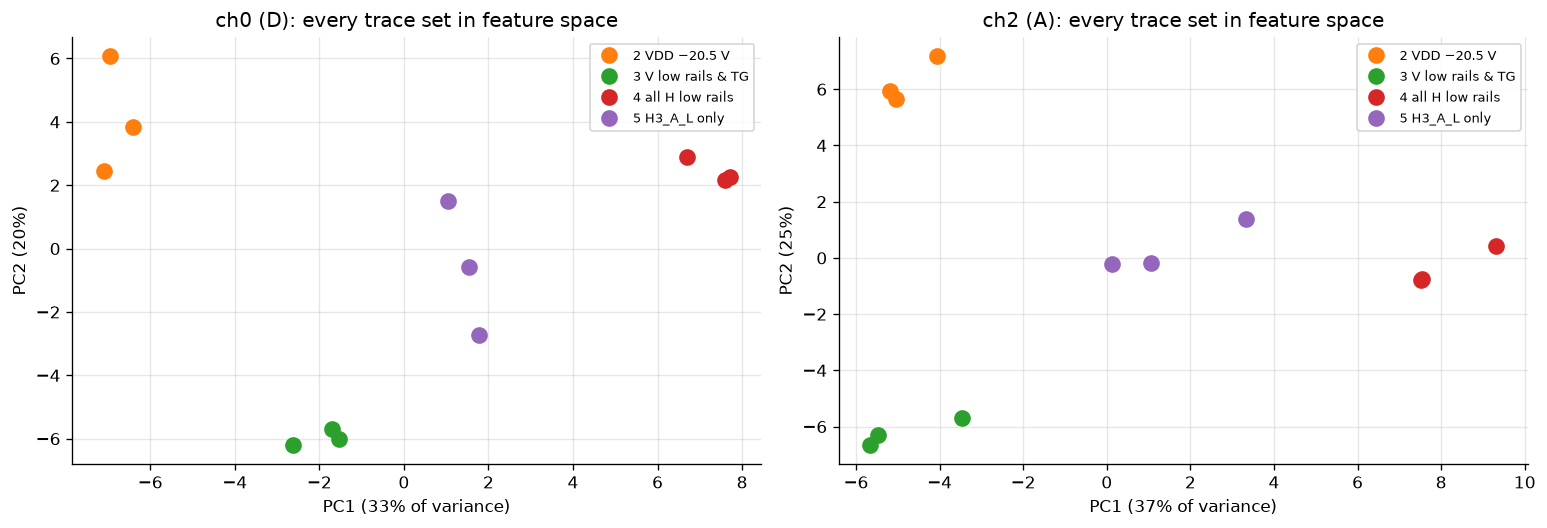
\includegraphics[width=\textwidth]{oct12_feature_space.png}
\caption{Every trace set (one dot each) projected onto the first two principal components of its standardized features.
Left: channel 0, right: channel 2. Each colour is one setting.}
\label{fig:space}
\end{figure}

\subsection{Is this enough to train the target model?}
\label{sec:ml-target}

No. This run was a test of the procedure, not a training set. What a training set needs, and why:

\begin{table}[H]
\centering
\begin{tabularx}{\textwidth}{>{\raggedright\arraybackslash}p{4.2cm}X>{\raggedright\arraybackslash}p{3.8cm}}
\toprule
Needed & Why & This run \\
\midrule
Many distinct parameter sets ($\sim$100) &
A model learns a function of $\theta$ from examples. With $d$ varied parameters, a common rule of thumb is at least
$10\,d$ examples (5--10 parameters $\to$ 50--100 packets) to fit even smooth trends, and more to see interactions. &
5 \\
\addlinespace
A design in which the effects can be separated &
If two parameters always change together, no model can tell which one caused a change. Example: from 5 to 2, both VDD and
H3\_A\_L change, so a change in the horizontal transfer could be due to either. Here only the physics argument
(VDD should not move the clocks) separates them. &
rails changed in blocks; VDD confounded with H3\_A\_L and with the trace setup \\
\addlinespace
Image labels for every packet &
The model predicts $\sigma_e$, $\lambda$ and the gain, so every example needs them. WADERs measures them by fitting the 0, 1,
2\,e$^-$ peaks, which needs unbinned (or low-charge) pixels. &
none: the 20$\times$20 bins hold 20--35\,e$^-$ \\
\addlinespace
Labels that vary &
If $\sigma_e$ is the same in every example, there is nothing to learn about what changes it. The parameter ranges must be wide
enough to move $\sigma_e$ and $\lambda$ measurably. &
image noise changed only in setting 3 (with an inverted rail) \\
\addlinespace
Repeated references &
The CCD and electronics drift over hours. Without the same reference setting measured again, a drift looks like an effect of
$\theta$. &
none; settings up to 85\,min apart \\
\bottomrule
\end{tabularx}
\end{table}

\subsection{What this run does provide}

\begin{enumerate}
\item \textbf{Evidence that trace features are good inputs.} They respond strongly (separations 10--700), each to its own
  parameter, and agree between repeats.
\item \textbf{A noise estimate for every feature} (the repeat scatter), needed for weighting the features.
\item \textbf{A first trace--image link}: the noise of amplifier A.
\item \textbf{Lessons for the data taking}: set every trace cut, take reference traces in every packet, and change one
  parameter (or a random combination) per packet over a range wide enough to move $\sigma_e$.
\end{enumerate}

\subsection{Next data}

Each packet is taken with \code{take\_packet.py}: 3 flushes, 3 reference trace sets (at the reference $\theta$), the new
$\theta$, a flush, 3 trace sets, and a 1$\times$1 image that WADERs can fit (Table~\ref{tab:image}). The reference traces in
every packet measure the drift directly, and \code{take\_packet.py} sets all trace cuts, so the \code{NCOLPRE} problem cannot
recur. At about 10 minutes per packet, an overnight run gives 80--100 packets. Suggested order:
\begin{enumerate}
\item \textbf{One parameter at a time:} about 5 parameters $\times$ 5 values (25 packets), with ranges wide enough to change
  $\sigma_e$. Each effect is then unambiguous (no confounding), and the scan shows whether it is linear, has an optimum, or
  has a threshold.
\item \textbf{A random design} over the same parameters (50--100 packets): every packet draws all parameters at random within
  their ranges. Because the parameters vary independently, a model can separate their effects and learn how they interact
  (e.g.\ whether the best VDD depends on the reset rails).
\item \textbf{The reference setting repeated every few packets}, to measure the drift over the night.
\end{enumerate}
With about 100 such packets, a Gaussian-process or small tree-ensemble model of $\sigma_e(\theta, \text{trace features})$
becomes meaningful. A Gaussian process also gives an uncertainty for every prediction, which an optimizer can use to choose
the next packet.

\begin{table}[H]
\centering
\begin{tabular}{ll}
\toprule
Parameter & Value \\
\midrule
\code{NROW} $\times$ \code{NCOL} $\times$ \code{NDCM} & 35 $\times$ 1000 $\times$ 200 \\
\code{NPBIN}, \code{NSBIN} & 1, 1 \\
\code{NCOLPRE} & 5300 (854 active + 146 overscan columns, as the 2026-10-06 1$\times$1 image) \\
\code{NROWPRE}, \code{NCOLPOST}, \code{NROWPOST}, \code{NDCMPRE} & 0 \\
\code{BOOLCLR}, \code{EXPOSURE} & 1, 10\,s \\
Readout & 8.11\,s per row $\to$ about 4.9\,min \\
Expected & $\sim$30,000 active pixels per channel; 0.05--0.1\,e$^-$/pix; $\sim$2,000--3,000 one-electron pixels \\
Noise & $\sigma \approx 0.23$\,e$^-$ on channel 0 (channel 2 $\approx 0.9$\,e$^-$) \\
WADERs & \code{img\_9.json} with \code{ccd\_rows} 35, \code{ccd\_cols} 854; dark current fitted per row \\
\bottomrule
\end{tabular}
\caption{Recommended 5-minute 1$\times$1 dark-current image (from the dark rate measured on 2026-10-12,
$4.4$--$6.7\times10^{-4}$\,e$^-$/pix/s).}
\label{tab:image}
\end{table}

%======================================================================
\section{Summary}

\begin{itemize}
\item Every parameter change moved 10--30 of the 85 trace features per channel, far beyond the repeat scatter.
\item The features moved are specific to the parameter: H rails $\to$ horizontal transfer, V rails/TG $\to$ vertical
  transfer, VDD $\to$ amplifier response.
\item The noise of amplifier A rose in both the trace and the image when the V rails and TG were lowered.
\item The features identify the setting of a trace set in 46 of 47 cases.
\item A model of $\sigma_e$, $\lambda$ and the gain needs about 100 packets with a proper design, reference traces and 1$\times$1
  images.
\end{itemize}

\paragraph{Sources.} Analysis: \code{notebooks/packet\_tests\_2026-10-12.ipynb}. Features: \code{src/trace\_features.py}
(described in \code{docs/trace\_features.tex}). Session notes: \code{docs/context/2026-10-12\_session\_context.md}.

\appendix
\section{All 85 features}

\begin{figure}[H]
\centering
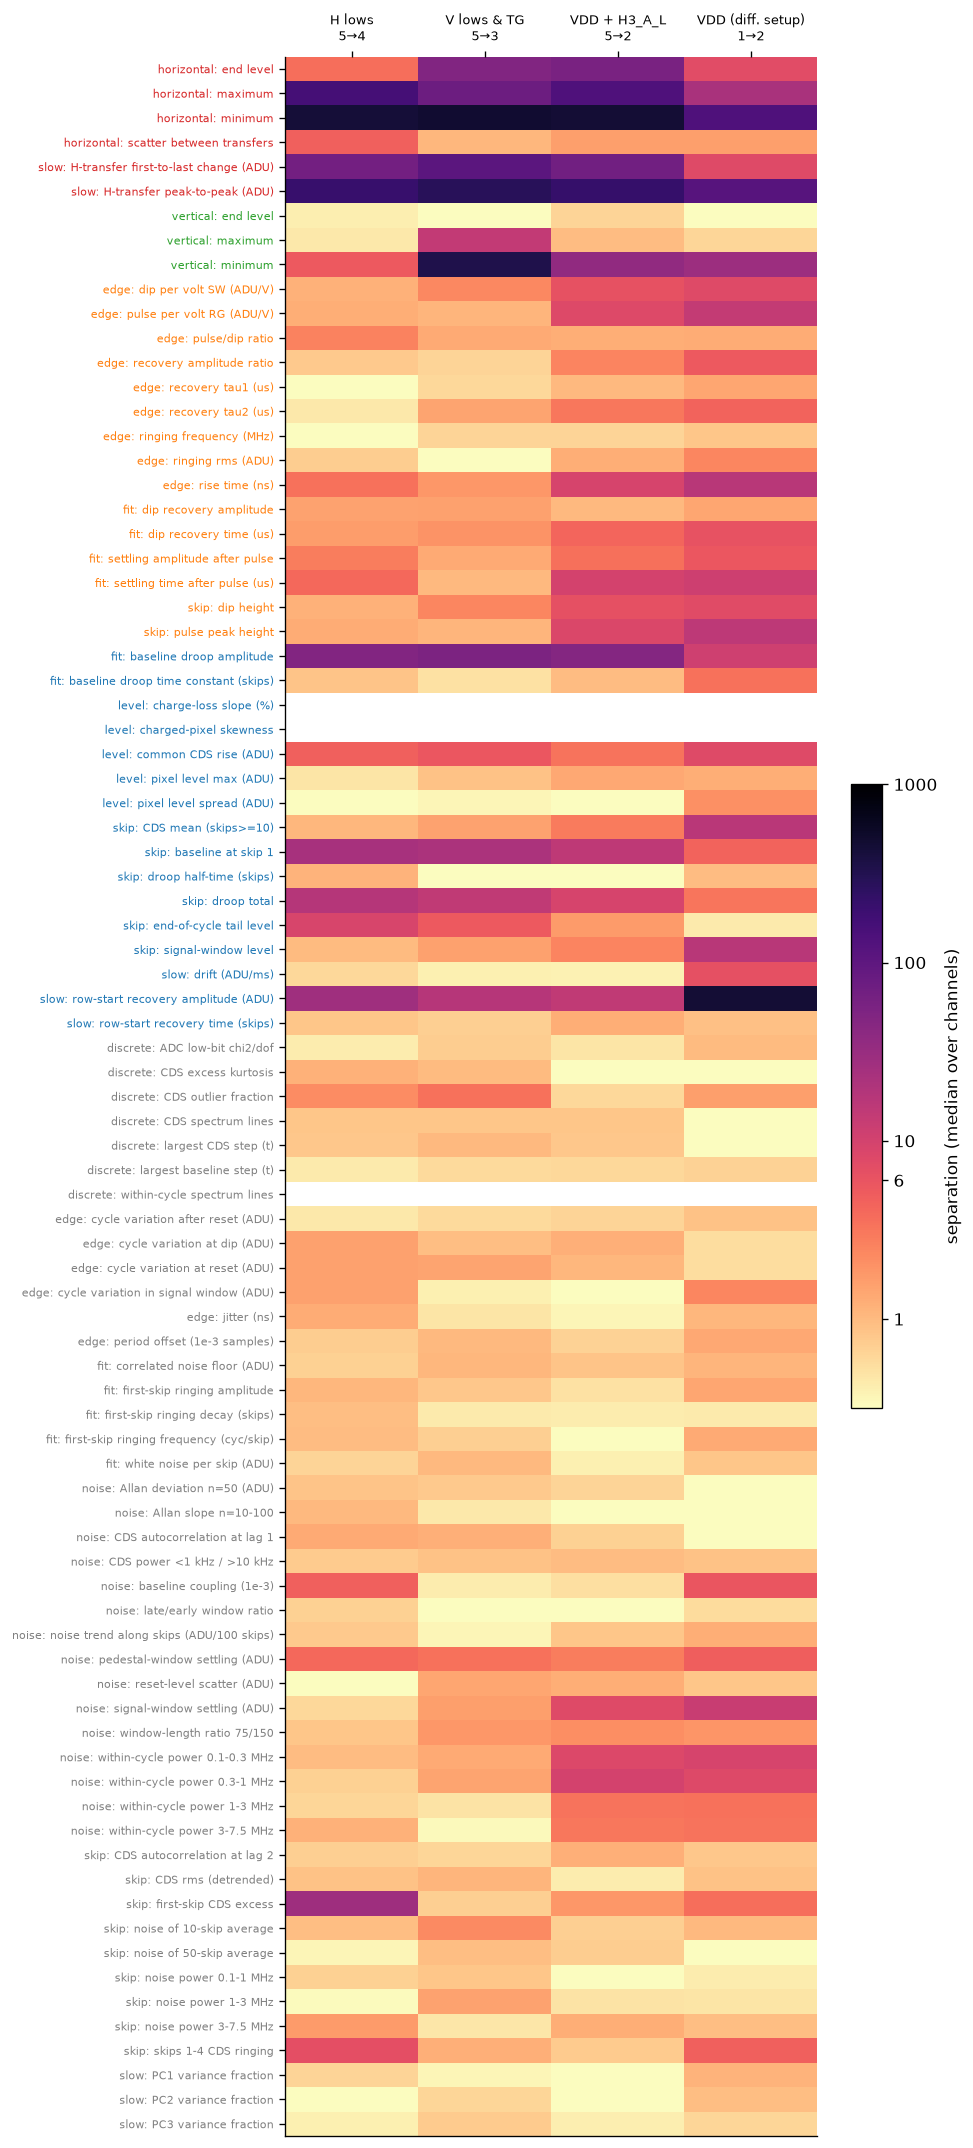
\includegraphics[height=0.85\textheight]{oct12_all_features.png}
\caption{Median separation over the 4 channels of every feature for four comparisons. Feature names are coloured by kind as
in Figure~\ref{fig:fingerprints}.}
\end{figure}

\end{document}
